% PLEASE USE THIS FILE AS A TEMPLATE FOR THE PUBLICATION
% Check file IOS-Book-Article.tex


% preferred topic area: algorithms
%
% at most 5 keywords
%
% relevance
%
% originality


\documentclass{IOS-Book-Article}     %[seceqn,secfloat,secthm]

\usepackage{mathptmx}
%\usepackage[T1]{fontenc}
%\usepackage{times}%
%
%%%%%%%%%%% Put your definitions here

\usepackage{amsmath,amssymb}
\usepackage{cite}
\usepackage{color}
\usepackage{graphicx}
\usepackage{url}
\usepackage{xspace}

\newcommand{\comment}[1]{\textcolor{green}{[DAC: #1]}\xspace}
\newcommand{\todo}[1]{\textcolor{red}{[TODO: #1]}\xspace}
\newcommand{\sR}{\mathbb{R}}
\newcommand{\dt}{\mathrm{d}t}
\newcommand{\clawpack}{{\sc Clawpack}\xspace}
\newcommand{\forestclaw}{Forestclaw\xspace}
\newcommand{\pforest}{\texttt{p4est}\xspace}
\newcommand{\manyclaw}{Manyclaw\xspace}


% \newcommand{\plotbox}[1]{\fbox{#1}}
\newcommand{\plotbox}[1]{#1}

\newcommand{\Fig}[1]{Figure~\ref{fig:#1}}

\newcommand{\alert}[1]{{\color{red}#1}}

%%%%%%%%%%% End of definitions
\begin{document}
\begin{frontmatter}          % The preamble begins here.
%
%\pretitle{}
\title{\forestclaw:
        Hybrid forest-of-octrees AMR for hyperbolic conservation laws}
\runningtitle{\forestclaw}
%\subtitle{}

% Two or more authors:
%\author[A]{\fnms{} \snm{}},
%\author[B]{\fnms{} \snm{}}
%\runningauthor{}
%\address[A]{}
%\address[B]{}
%
\author[A]{\fnms{Carsten} \snm{Burstedde}%
\thanks{Corresponding author.  E-mail: \texttt{burstedde@ins.uni-bonn.de}}},
\author[B]{\fnms{Donna} \snm{Calhoun}},
\author[C]{\fnms{Kyle} \snm{Mandli}} and
\author[C]{\fnms{Andy R.} \snm{Terrel}}
\runningauthor{C.\ Burstedde et al.}
\address[A]{Institut f\"ur Numerische Simulation, Universit\"at Bonn, Germany}
\address[B]{Boise State University, Idaho, USA}
\address[C]{Institute for Computational Engineering and Sciences,\\
The University of Texas at Austin, USA}

\begin{abstract}
We present a new hybrid paradigm for parallel adaptive mesh
refinement (AMR) that combines the scalability and lightweight architecture of
tree-based AMR with the computational efficiency of patch-based solvers for
hyperbolic conservation laws.  The key idea is to interpret each leaf of the AMR
hierarchy as one uniform compute patch in $\sR^d$ with $m^d$ degrees of freedom,
where $m$ is customarily between 8 and 32.  Thus, computation on each patch can
be optimized for speed, while we inherit the flexibility of adaptive meshes.  In
our work we choose to work with the \pforest AMR library since it allows us to
compose the mesh from multiple mapped octrees and enables the cubed sphere and
other nontrivial multiblock geometries.
\end{abstract}

\begin{keyword}
adaptive mesh refinement,
hyperbolic conservation laws,
clawpack,
HPC,
manycore
\end{keyword}

\end{frontmatter}

%%%%%%%%%%% The article body starts:

\section{Introduction}

With the advent of many-core chips, such as GPUs and the MIC architecture, comes the opportunity to sustain unprecedented rates of floating point
operations at comparably high integration density and low cost.  These
architectures, however, require careful structuring of the data layout and
memory access patterns to exhaust their multithreading and vectorization
capabilities.

Consequently, it is not clear a priori how to accelerate PDE solvers
that use adaptive mesh refinement.
%, especially when working with
%unstructured meshes \comment{This sounds we are now going to talk
%  about unstructured meshes.}.
% CB: Good point, took it out.
Of course, it was realized early that it helps to aggregate degrees of
freedom (DOF) at the element level, as has been done with high-order
spectral element \cite{TufoFischer99}, low order continuous Galerkin methods that accumulate many elements simultaneously \cite{knepleyterrel:2013},
%finite volume (element?)
or discontinuous Galerkin \cite{HesthavenWarburton02}
methods.  GPU implementations of the latter have been proposed recently
\cite{KlocknerWarburtonBridgeEtAl09, BursteddeGhattasGurnisEtAl10}.
The finite volume method has typically been implemented using a single degree
of freedom per cell on
% either
structured
\cite{ppm, clawpack}
or unstructured meshes
\cite{openfoam};
higher order methods have also been constructed by widening the stencil, for instance in WENO methods
\cite{Shu:2009bi}.
% \comment{Are you looking for
%   references to parallel AMR codes?  Or more general AMR codes based
%   on the FVM?}  \todo{No, I was looking for unstructured FV
%   references.  Would you have any, and can we add the block-AMR
%   references later?} \comment{But most finite volume methods
%   (structured or unstructured) only have a single degree of freedom
%   per mesh cell (``element''?)  Only recently have people increased
%   the order by extending the stencil (without increase the DOFs per
%   mesh cell).}
% CB: Can you fix some of the above citations?

% For example, SEs optimized for computational speed have originally been
% implemented on unstructured conforming meshes \cite{TufoFischer99} and later
% been extended to non-conforming adaptive meshes \cite{FischerKruseLoth02,
% BursteddeGhattasGurnisEtAl10}.

To facilitate hardware acceleration for parallel dynamic AMR, we
build upon the forest-of-octrees paradigm because of its low overhead
and proven scalability \cite{BursteddeWilcoxGhattas11}.  This approach
identifies each octree leaf with a mesh element.  \alert{The presented work goes beyond the traditional high-order element and defines each element to
be a dense computational patch with $m^d$ DOFs.}  In fact, this approach
resembles block-structured AMR \cite{be-ol:1984, be-co:1989,
% be-le:1991 (cited below)
ColellaGravesKeenEtAl07,
BerzinsLuitjensMengEtAl10} except that the
patches are not overlapping,
% (except in ghost cell regions),
% CB: we comment on this later in Section 4.
which enables us to capitalize on our
previous experience with scalable FE solvers for PDEs
\cite{BursteddeStadlerAlisicEtAl13}.  The \clawpack software
\cite{LeVeque97} provides a popular implementation of such a patch.
It has been designed to solve hyperbolic conservation laws
% on a uniform compute patch
and successfully used in the context of block-structured AMR
\cite{be-le:1991, amrclaw, Berger:2011du}.
\comment{Review 1 points out that the statement in red may not be what we are intending to say here.  Mainly the distinction between claiming better convergence then a high-order method (which I think is not what we are saying) and just stating that our elements are patches themselves as opposed to a single DOF.}

In this paper we describe our design for the coupling of forest-of-octree AMR
with \clawpack at the leaf level.  We comment on challenges that arise in
enabling multiblock geometries and efficient parallelism and conclude with a range
of numerical examples that demonstrate the conceptual improvements in relation
to other approaches.

\section{Design principles}

The starting point of our work is defined by the \pforest algorithms for
forest-of-octrees AMR on the one hand, and the \clawpack algorithms for the
numerical solution of hyperbolic conservation laws
% on uniformly gridded domains
on the other.  Both are specialized codes with the following characteristics:
% \comment{I am not sure about the Python dependency;  the latest version of
% \clawpack relies on
%Python to generate an input file, but the code itself is F77 (or maybe some
%F90). }
% CB: I made it optional.
% DAC: Good.
\begin{center}
\begin{tabular}{l|l|l}
& \multicolumn{1}{c|}{\pforest} & \multicolumn{1}{c}{\clawpack} \\
\hline
subject & hexahedral nonconforming mesh &  hyperbolic PDE on $[0, 1]^d$ \\
toplevel unit & forest of octrees & patch of $m^d$ FV cells \\
atomic unit & octree leaf & one DOF in each cell \\
parallelization & MPI & threads (\manyclaw variant) \\
memory access & distributed & shared on each MPI rank \\
data type & integers & floating point values \\
language & C & Fortran 77 \\
% CB: dropped dependencies.
% dependencies & none & Python (optional) \\
%\hline
\end{tabular}
\end{center}
Each leaf as the atomic unit of \pforest houses a toplevel unit of \clawpack.
The term cell is used to identify a single DOF within a \clawpack patch.  The
proposed 1:1 correspondence between a leaf and a patch thus combines two
previously disjoint models in a modular way:
\begin{enumerate}
\item We permit the reuse of existing, verified, and performant codes.
% if the integration is done well
\item We preserve the separation between the mesh on one hand and the
discretization and solvers on the other.
\item The AMR metadata (\pforest:
under 1k bytes per octree, 8 bytes per MPI rank,
24 bytes per leaf. \forestclaw: $84 + 28d$ bytes per patch)
% \comment{?? : in 3d: 5 ints,  9 floats; in 2d: 4 ints, 6 floats}
% CB: thanks, I have added it.
is insignificant compared to
the numerical data ($m^d$ floating point values per patch).
\item The resulting parallel programming model is a hybrid (often referred
to as MPI+X).  Only rank-local leaves/patches are stored and computed on.
\end{enumerate}

% yields periodicity as a special case
A particular feature of \forestclaw is that the generic handling of multiblock
geometries is inherited from \pforest, identifying each octree as a block.
% and each leaf as a patch.
Each block is understood as a reference unit cube with
its own geometric mapping.  The connectivity of the blocks can be created by
external hexahedral mesh generators, eliminating the need to encode it by hand.

A main challenge is presented by the fact that the patch neighborhood
is only known to \pforest.  This patch connectivity information needs
to be propagated to the numerical code in \forestclaw that implements
the interaction with neighbor patches via the use of a layer of ghost
cells surrounding each patch.  \alert{To this end}, we define an interface
that allows read-only access to the sequence of blocks,
the list of patches for each, and a lookup of neighbor patches (and
their relative orientation which is nontrivial between blocks).
Suitably informed by \pforest, \forestclaw stores only the patches local to
each MPI rank.  \alert{The exchange of ghost} data and parallel repartitioning is
provided transparently by \pforest.  Mesh modification directives, such as
adaptive refinement and coarsening, are called from \forestclaw and relayed to
\pforest.

\alert{Review 2 requests more info on how this is done.  Sounds like they are more curious about the refinement overhead to other leaves on the tree and the strategy as to how refinement is decided.}

% Forestclaw would support swapping out p4est or \clawpack


% AMR Metadata $\ll$ numerical data

% Experience from integration with large-scale adaptive-mesh PDE solvers.
% Design goals: Lightweight, modular, reuse.

% Mesh information is discrete (tree nodes have integer coordinates in
% $(0, 2^L($ where $L$ is the maximum allowed refinement level of the tree.

% Dimension independence

% rank as is common with parallelization using the MPI framework
% \cite{Forum94, SnirOttoHuss-LedermanEtAl96}.

\section{Parallelization}

\begin{figure}
\begin{center}
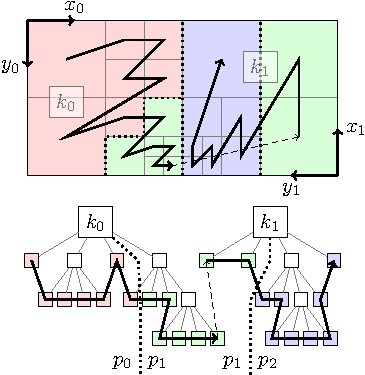
\includegraphics[width=.4\columnwidth]{../figs_misc/forest_stacked}
\hspace{.05\columnwidth}
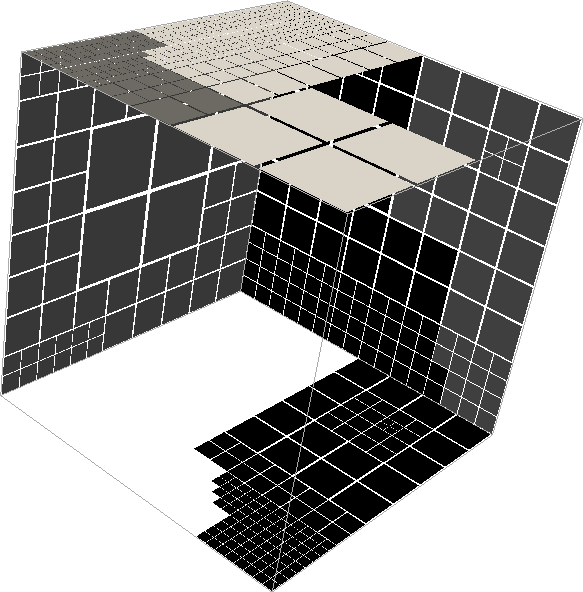
\includegraphics[width=.4\columnwidth]{../figs_misc/cubed3}
\end{center}
\caption{Left: Forest of two quadtrees, partitioned among three MPI processes.
Each quadtree has its own coordinate orientation.  The situation in 3D
(octrees) is analogous.  Right: The leaves in a forest of six quadtrees that
serves as the computational domain for the cubed sphere.  An adhoc refinement
pattern has been 2:1 balanced in terms of neighbor sizes and partitioned
between five MPI processes (the three middle ones are shown from black to
white).}
\label{fig:cubed3}
\end{figure}

The MPI layer is addressed from within \pforest and not exposed to the
\forestclaw code.  The order of leaves is maintained in \pforest according to a
space filling curve.  Each MPI rank has a local view on its own partition,
augmented where necessary with information about one layer of ghost leaves
(see \Fig{cubed3}).

\forestclaw uses iterators over all rank-local leaves, optionally restricted to
a given level.  Random access is possible and used when executing $O(1)$ time
neighbor lookups.  Looping over the patches in the order prescribed by the
forest
\alert{Review 2 - Explain the preceding paragraph in more detail}
% \comment{tree?}
% CB: I think forest is fine here.
and
accessing neighbors only relative to the current patch leads to a high
percentage of cache reuse
\cite{BursteddeBurtscherGhattasEtAl09}.
% since the ghost patches are likely closeby with respect to the $z$-order.

When \forestclaw accesses neighbor patches, they can be on the same or a
different block.  In the latter case, coordinate transformations are carried
out.  The structure of \forestclaw is oblivious to the fact that it only has a
local view of the distributed mesh and data which relieves the developer from
programming to the MPI interface.  Parallel neighbor exchanges are hidden
inside \pforest and called by \forestclaw at well-defined synchronization
points.  There is one such parallel data exchange per time step for a global
value of $\dt$, the time step length, or one exchange per discretization level per time step if $\dt$
is chosen per-patch depending on its size (this is sometimes called
sub-cycling).  When using sub-cycling, the load balance is attained per level as
it is done for example in Chombo \cite{ColellaGravesKeenEtAl07}
or recent geometric adaptive multigrid schemes
\cite{SundarBirosBursteddeEtAl12}.

The threaded parallelism over the degrees of freedom of a patch can be handled
by \forestclaw alone without the need to involve \pforest.  Additionally many-core implementations, such as \manyclaw \cite{manyclaw}, can be used for the integration of the hyperbolic system on a leaf-patch thereby allowing for hybrid parallelism.  The design of leaf-patches then can enable efficient management of data local to many-core architectures (e.g. the Xeon Phi), and the host.

% Trees have different coordinate systems.
% neighbor block: permutation of patch points due to non-aligned coordinate
% systems

% neighbor rank: data needs to be fetched over the network first.

% $L$ is 30 for 2D and 19 for 3D, so it allows for deep hierarchies.

% fast (O(log N/P)) neighbor and parent/child lookups
% horizontal/vertical tree traversal

% \todo{What is BearClaw (tree-based / S.\ Mitran)?}

\section{Patch-based numerics at the leaf level}

% CB: I'm trying to avoid "mesh" cell here since in \pforest FE simulations
% that would mean a whole leaf.

For hyperbolic problems, we integrate the solution on a single uniform patch,
containing $m^d$ cells, using the wave propagation algorithm described by R. J.
LeVeque \cite{LeVeque:1997eg} and implemented in \clawpack \cite{le:2002,
clawpack}.  We assume a single degree of freedom per cell and reconstruct a
piecewise constant solution to obtain left and right states at cell edges.  At
each edge, we solve Riemann problems to obtain left and right going waves
propagating at speeds determined from the solution to the Riemann problem.  For
scalar advection, the speed of each wave is simply the local advection speed at
the cell interface.  For non-linear problems and systems, an approximate
Riemann solver, such as a Roe solver \cite{roesolver}, is typically used.  Since
much of the physics of an application can be contained in the Riemann solver,
\forestclaw adopts \clawpack's interface to Riemann solvers effectively allowing
problems solved with \clawpack to be solvable in \forestclaw.  In order to
achieve second order accuracy wave limiters are used to suppress spurious
oscillations at sharp gradients in the flow.

Data exchanges between neighboring patches are done via layers of
ghost cells extending the dimensions along the edges of each patch.
The interior edge values of a given patch overlap the ghost cell
region of a neighboring patch.  For the second order wave propagation
algorithm, two layers of ghost cells are sufficient.  This implies that
one layer of ghost patches is sufficient for $m \ge 4$.  Neighboring
patches at the same level of refinement simply copy their interior
edge values into a neighbors' ghost cells.  Neighboring fine grid
patches average their interior edge data to a coarser neighbor's ghost
cell values.  And neighboring coarse grid patches interpolate data
from their interior edge cells to their fine grid neighbor's ghost
cell values.  To avoid loss of conservation and the creation of
spurious extrema, we use a standard conservative, limited
interpolation scheme to interpolate values from the coarse grid to
fine grid coarse cells \cite{amrclaw, chombo}.  When sub-cycling, time accurate
data between coarse grids is used to fill in ghost cells for fine grids.
As mentioned in the previous section, this procedure can be extended
transparently to distributed parallelism by defining an abstract exchange
routine for ghost patch data.

Grid refinement and coarsening requires interpolation from coarse grids
to newly created fine grids, and the averaging of fine grid data to a newly
created underlying coarse grid.  This operation is rank-local, analogous to the
general dynamic AMR procedures used in \pforest-based FE codes \cite[Fig.\
4]{BursteddeGhattasStadlerEtAl08}.

\section{Numerical results}

\begin{figure}
\begin{center}
\plotbox{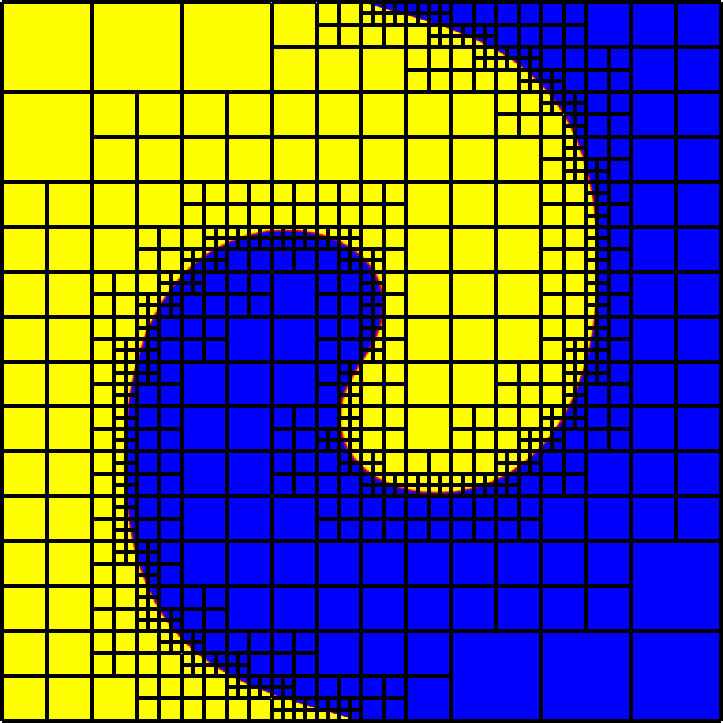
\includegraphics[width=.4\columnwidth]{quadtree}}
\hspace{.05\columnwidth}
\plotbox{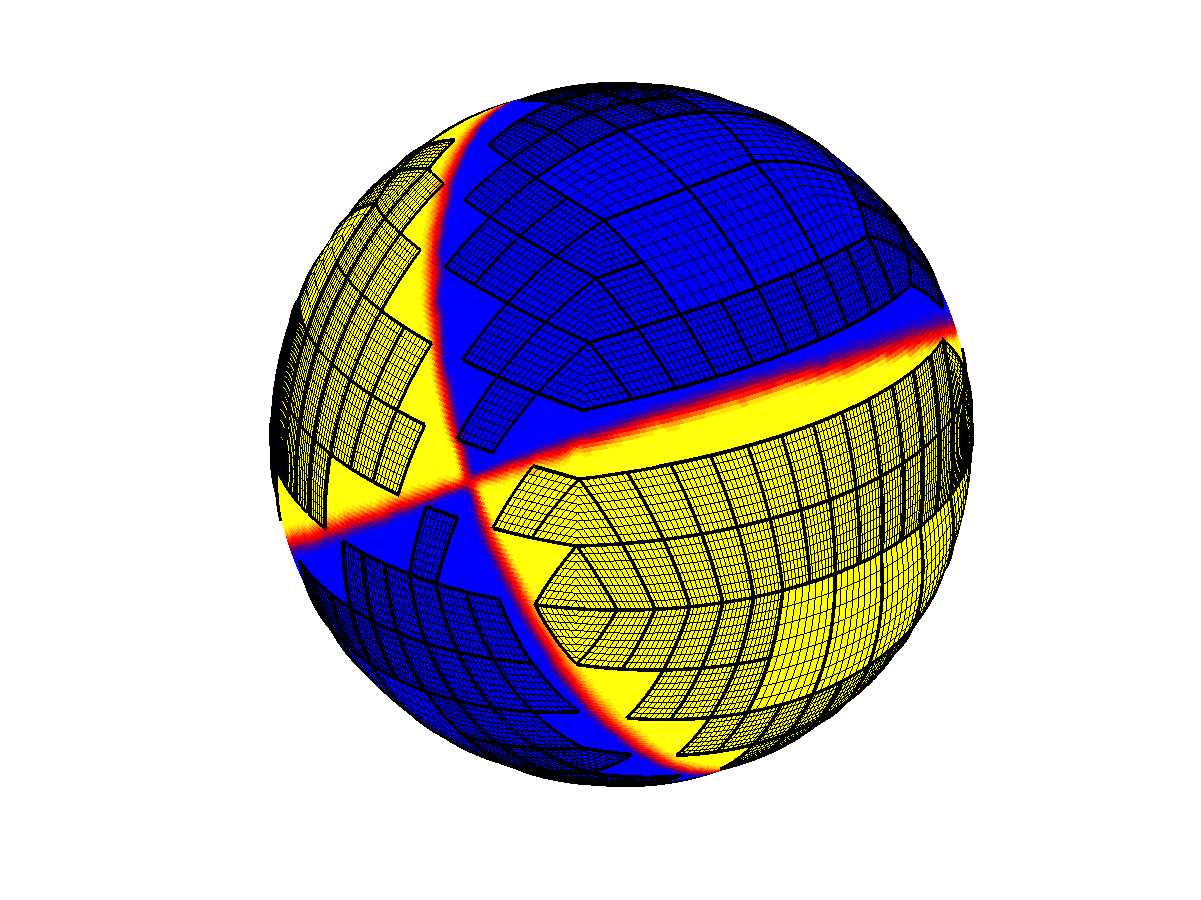
\includegraphics[width=.4\columnwidth]{sphere_plot167}}
\end{center}
\caption{Numerical results for solving the advection equation.  Left:  Unit
square (single quadtree) with a twisting velocity field.  Right: Spherical ball
with a rotational velocity field constructed from two mapped quadtrees.  In
both cases the concentration is color-coded with a sharp gradient shown in red.
The adaptive mesh refinement follows the location of the gradient (the patches
are not shown where they become too fine for display).  Here we use $m = 8$
cells per \clawpack patch.}
\label{fig:results2d}
\end{figure}

We provide two examples that demonstrate the \forestclaw code.
The numerical results to date have been designed to verify that
interface layer between \pforest and \forestclaw is sufficiently
flexible and robust.  Of particular importance was ensuring that all
ghost cell transfers (including averaging and
interpolation) have been implemented correctly.
The basic \clawpack algorithm and corresponding code have been
thoroughly tested and need no further verification in our context.

In both sets of numerical results, we solve a scalar advection
equation,
\begin{equation}
q_t + ({\bf u}\cdot \nabla) q = 0 ,
\end{equation}
where the velocity field ${\bf u} = (u(\xi,\eta,t), v(\xi,\eta,t)$ is
a prescribed function of computational coordinates.  The relevant
numerical parameters that are set in each case include the size of the
patch on each leaf ($m=8$ in each case), and the minimum and maximum
refinement levels, which in turn fix minimum and maximum effective grid
resolutions.

In both examples, a patch is tagged for refinement if the
difference between its maximum and minimum values exceeds a prescribed
threshold.  A family of $2^d$ patches is coarsened to a parent patch
if this patch would not meet the criteria for refinement.

\begin{description}
\item{\bf Example 1:} An initial concentration field $q$
is set to 0 in the left half of a computational square and to 1 in the
right half.  A time dependent flow field is prescribed that distorts
the interface between the 0 and 1 concentration values.  The minimum
and maximum levels of refinement are set to 3 and 6, respectively.
This results in a minimum resolution of $64 \times 64$ and a maximum
resolution of $512 \times 512$.  \Fig{results2d} shows the results
at an intermediate time step.

% \begin{figure}
% \begin{center}
% \plotbox{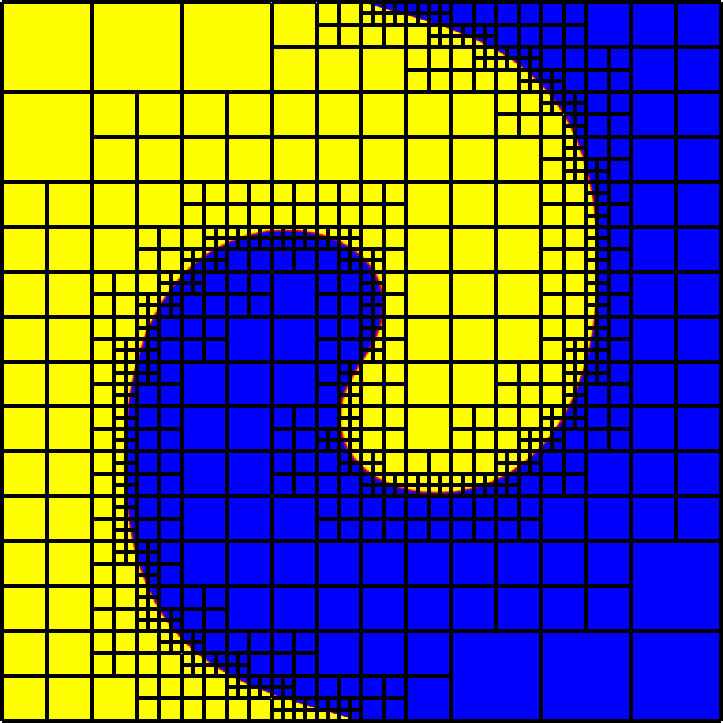
\includegraphics[height=0.485\textwidth,clip=true,trim=3cm 0cm 2cm 0cm]{quadtree.png}} \hfil
% \plotbox{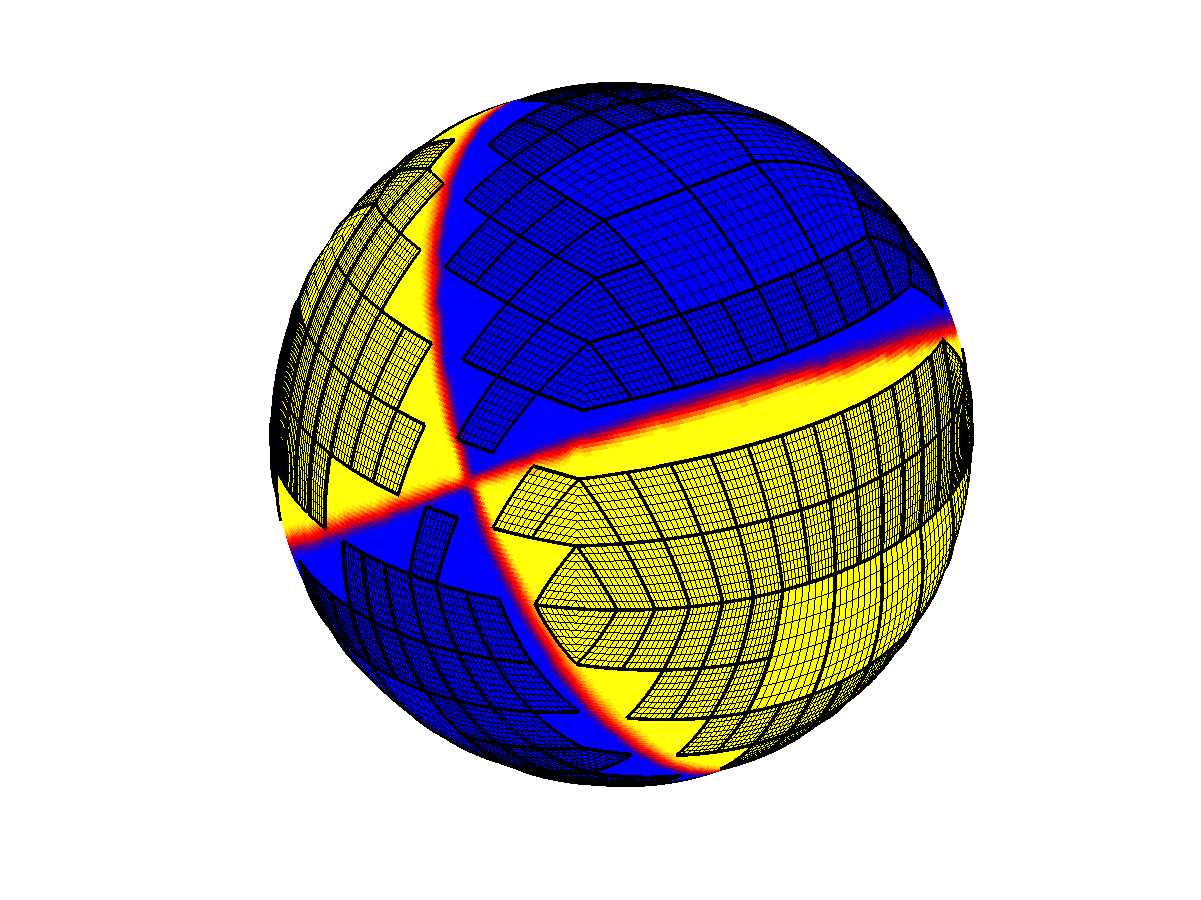
\includegraphics[height=0.485\textwidth,clip=true,trim=6cm 0cm 7cm 0cm]{sphere_plot167.png}}
% \end{center}
% \caption{Results for scalar advection using \forestclaw.}
% \label{fig:results}
% \end{figure}

\item{\bf Example 2:} We demonstrate the
multiblock functionality of \forestclaw by considering flow on a
sphere.  The sphere mapping we use consists of two quadtrees, each
defined in the computational space $[-1,1] \times [-1,1]$
\cite{ca-he-le:2008, be-ca-he-le:2009}.  Each quadtree is mapped to cover one
hemisphere.  The initial conditions is $q = 0$ in one half of
the sphere, and $q = 1$ in the other half, where the halves are not
necessarily aligned with the equator of the mapping.  The flow field
${u}$ simulates rigid body rotation.  We show the results at an intermediate
time in \Fig{results2d}.
\end{description}

The results in this section are preliminary and will be extended in the final
version.  We have so far exercised \forestclaw for two 2D manifolds,
% namely the
% unit square and a sphere composed of two mapped squares.
% On both we solve the
% advection equation with a given velocity field.
advecting a concentration field with a sharp gradient that we track dynamically
with adaptive mesh refinement.  We observe that the refinement follows the
front and allows for an accurate representation of its location over time.
% \Fig{results2d}.

\pforest is parallelized with MPI and well tested on large supercomputers, both
in 2D and 3D.  Parallelization of \forestclaw is not completed yet but
envisioned for the final version of the paper.

\section*{Acknowledgements}

The authors acknowledge valuable discussion with Randy LeVeque, Marsha
Berger, and Hans-Petter Langtangen.  We also acknowledge David
Ketcheson and the KAUST sponsored HPC$^3$ numerics workshop at which
the initial phases of this project were first discussed.  The second
author would like to also acknowledge the Isaac Newton Institute
(Cambridge, UK), where much of the preliminary development work for
\forestclaw was done. The leaf/patch paradigm was independently
presented by B.\ as part of a talk at the SCI Institute, Salt Lake City, Utah,
USA in July 2011.


%%%%%%%%%%% The bibliography starts:
\bibliographystyle{unsrt}
\bibliography{../biblio/ccgo,../biblio/amr}

\end{document}
